\section*{Einführung}

Ein \textbf{Prisma} ist ein Körper mit zwei kongruenten, parallelen Grundflächen.\\
Die Formel für das \textbf{Volumen} eines Prismas lautet:
\[
V = G \cdot h
\]
Die Formel für die \textbf{Oberfläche}:
\[
O = 2 \cdot G + M
\]
Dabei ist:
\begin{itemize}
  \item \( G \) die Fläche der Grundseite,
  \item \( h \) die Höhe des Prismas,
  \item \( M \) die Mantelfläche (Summe aller Seitenflächen).
\end{itemize}




\vspace{1cm}


\section*{Aufgabe 2: Dreiecksprisma}

Berechne Volumen und Oberfläche.

\begin{center}
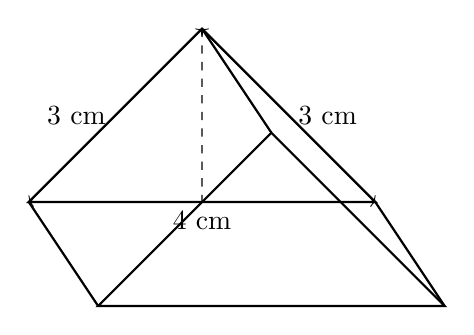
\begin{tikzpicture}[scale=1.1]
  % Vorderes Dreieck
  \coordinate (A) at (0,0);
  \coordinate (B) at (4,0);
  \coordinate (C) at (2,2);
  % Hinteres Dreieck (verschoben)
  \coordinate (A') at (0.8,-1.2);
  \coordinate (B') at (4.8,-1.2);
  \coordinate (C') at (2.8,0.8);
  % Kanten vorn
  \draw[thick] (A) -- (B) -- (C) -- cycle;
  % Kanten hinten
  \draw[thick] (A') -- (B') -- (C') -- cycle;
  % Verbindungskanten
  \draw[thick] (A) -- (A');
  \draw[thick] (B) -- (B');
  \draw[thick] (C) -- (C');
  % Maße
  \draw[<->] (A) -- node[below] {4 cm} (B);
  \draw[<->] (B) -- node[right] {3 cm} (C);
  \draw[<->] (C) -- node[left] {3 cm} (A);
  % Höhe (optional)
  \draw[dashed] (B) -- (2,0);
  \draw[dashed] (C) -- (2,0);
  \node[below] at (2,0) {};
\end{tikzpicture}
\end{center}

\vspace{1cm}

\textbf{Volumen:} \\
\textbf{Oberfläche:} 

\newpage

\section*{Aufgabe 3: Sechseckprisma (regelmäßig)}

Ein regelmäßiges Sechseck hat eine Seitenlänge von 2 cm. Die Höhe des Prismas beträgt 5 cm.

\begin{center}
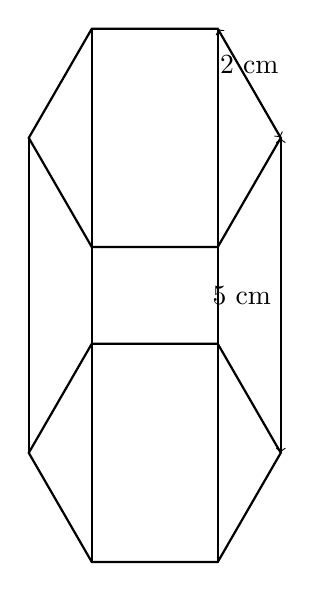
\begin{tikzpicture}[scale=0.8]
  % Grundfläche unten
  \foreach \i in {0,...,5} {
    \coordinate (G\i) at ({2*cos(60*\i)},{2*sin(60*\i)});
    \coordinate (H\i) at ({2*cos(60*\i)},{2*sin(60*\i)-5});
  }
  % Grundfläche
  \draw[thick] (G0) \foreach \i in {1,...,5} {-- (G\i)} -- cycle;
  % Deckfläche
  \draw[thick] (H0) \foreach \i in {1,...,5} {-- (H\i)} -- cycle;
  % Seitenkanten
  \foreach \i in {0,...,5} {
    \draw[thick] (G\i) -- (H\i);
  }
  % Beschriftung
  \draw[<->] (G0) -- node[above] {2 cm} (G1);
  \draw[<->,dashed] (G0) -- node[left] {5 cm} (H0);
\end{tikzpicture}
\end{center}

\vspace{1cm}

\textbf{Volumen:} \\
\textbf{Oberfläche:} 

\vspace{1cm}

\section*{Aufgabe 4: Schrägprisma (frei konstruiert)}

Berechne die fehlenden Größen. Ein Prisma hat ein Rechteck als Grundfläche mit \( a = 6\,\text{cm} \), \( b = 2\,\text{cm} \). Die schräge Höhe beträgt \( h = 5\,\text{cm} \).

\begin{center}
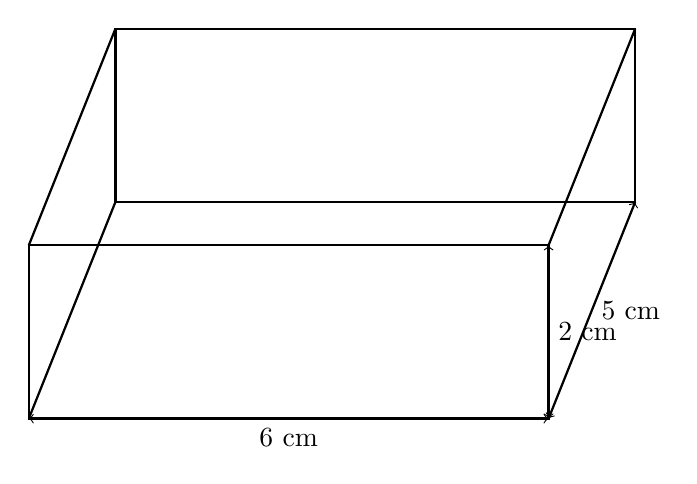
\begin{tikzpicture}[scale=1.1]
  % Grundfläche vorne
  \coordinate (A) at (0,0);
  \coordinate (B) at (6,0);
  \coordinate (C) at (6,2);
  \coordinate (D) at (0,2);
  % Grundfläche hinten (schräg)
  \coordinate (A') at (1,2.5);
  \coordinate (B') at (7,2.5);
  \coordinate (C') at (7,4.5);
  \coordinate (D') at (1,4.5);
  % Vorderes Rechteck
  \draw[thick] (A) -- (B) -- (C) -- (D) -- cycle;
  % Hinteres Rechteck
  \draw[thick] (A') -- (B') -- (C') -- (D') -- cycle;
  % Verbindungskanten
  \draw[thick] (A) -- (A');
  \draw[thick] (B) -- (B');
  \draw[thick] (C) -- (C');
  \draw[thick] (D) -- (D');
  % Maße
  \draw[<->] (A) -- node[below] {6 cm} (B);
  \draw[<->] (B) -- node[right] {2 cm} (C);
  \draw[<->,dashed] (B) -- node[right] {5 cm} (B');
\end{tikzpicture}
\end{center}

\vspace{1cm}

\textbf{Volumen:} \\
\textbf{Oberfläche:}

\vspace{1cm}
\textbf{Tipp:} Das Volumen berechnet sich unabhängig von der Schräge wie bei einem geraden Prisma.

\newpage

\section*{Aufgabe 5: Knobelaufgabe}

Ein rechteckiges Prisma hat eine Höhe von 10 cm und ein Volumen von 400 cm³. Die Länge der Grundseite beträgt 8 cm. Wie breit ist die andere Seite der Grundfläche?

\vspace{1cm}
\textbf{Rechnung:} 

\vspace{0.5cm}
\textbf{Lösung:}
